\chapter{Lenguaje: MSCLan}
\label{ch:lenguaje}
\lstsetpt

La herramienta \textit{Progtalk} debe recibir la comunicación que el
usuario desee procesar en un fichero escrito en un determinado
lenguaje que permita representar MSCs. Nosotros hemos creado uno
especificamente para este problema, y lo hemos bautizado como
\textit{MSCLan}. 

Nuestro lenguaje consta de dos secciones:
\begin{itemize}
\item Declaración de instancias, y
\item declaración de mensajes.
\end{itemize}

Cada una de estas declaraciones se llama sentencia, y entre sentencias
debe aparecer un símbolo '';'' que ejerce de separador.

\section{Instancias}

Las instancias de nuestro lenguaje se describen mediante tres
parámetros:

\begin{itemize}
\item Identificador de instancia. Este parámetro debe ser
  obligatoriamente introducido por el usuario. Ademas debe ser un
  identificador válido (aquí se entiende como identificador valido un
  conjunto de caracteres y números que comienza obligatoriamente por
  una letra).
\item Tipo de la instancia. Este parámetro es opcional, y esta pensado
  darle una funcionalidad real en un futuro desarrollo.
\item Parámetro \textit{name}. Este parámetro es opcional, y esta
  pensado darle una funcionalidad real en un futuro desarrollo.
\end{itemize}

El formato del lenguaje es:

\begin{itemize}
\item \lstinline[mathescape]!instance $iid$ of $tid$ { $name$ }!
\end{itemize}
donde:
\begin{itemize}
\item \lstinline{instance}, \lstinline{of}, ``\lstinline!{!'' y
    ``\lstinline!}!'' son palabras reservadas del lenguaje, y
\item $iid$ (identificador de instancia), $tid$ (tipo de la
  instancia), y $name$ (nombre del parámetro) deben ser introducidos
  por el usuario.
\end{itemize}

Algunos ejemplos de declaración de instancias son:

\begin{lstlisting}
instance a { "A" };
instance b of type { "B" };
instance c of control;
instance d;
\end{lstlisting}

El usuario puede almacenar tantas instancias como desee, pero estas
deben tener un identificador de instancia único.

A continuación mostramos un ejemplo gráfico de como representamos
gráficamente las instancias:

%\begin{figure}
%  \centering
%  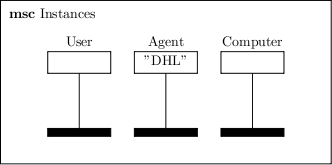
\includegraphics[scale=1]{./images/instances.pdf}
%  \caption{Ejemplo de representación gráfica de instancias.}
%  \label{fig:fig6}
%\end{figure}

\section{Mensajes}

Los mensajes de nuestro lenguaje se describen mediante seis
parámetros:

\begin{itemize}
\item Identificador de mensaje: este parámetro es opcional. En caso de
  ser introducido debe ser un identificador válido (aquí se entiende
  como identificador válido cualquier conjunto de letras, números y
  ''\_'' que comience por una letra,
\item Mensaje: este parámetro es opcional, y almacena el mensaje de
  texto propiamente dicho. Puede ser cualquier conjunto de caracteres
  salvo las comillas y que empiece y termine por comillas,
\item Instancia origen del mensaje: este parámetro debe ser
  obligatoriamente introducido por el usuario, y representa la
  instancia que envió el mensaje. La instancia a la que se haga
  referencia en este parámetro, debe de haber sido declarada
  previamente en esa misma comunicación,
\item Instancia destino del mensaje: este parámetro debe ser
  obligatoriamente introducido por el usuario, y representa la
  instancia que recibió el mensaje. La instancia a la que se haga
  referencia en este parámetro, debe de haber sido declarada
  previamente en esa misma comunicación,
\item Tiempo de envío: este parámetro es opcional. Representa el
  momento exacto en que el mensaje fue enviado, y
\item Tiempo de recepción: este parámetro es opcional. Representa el
  momento exacto en que el mensaje fue enviado.
\end{itemize}

El formato del lenguaje es:

\begin{itemize}
\item \lstinline[mathescape]!message $mid$ { $sms$ } from $orig$ @ $tsend$ to $dest$ @ $trec$!
\end{itemize}

donde,
\begin{itemize}
\item \lstinline{message}, \lstinline{from}, \lstinline{to},
  ''\lstinline{@}'', ``\lstinline!{!'' y ``\lstinline!}!'' son
  palabras reservadas del lenguaje, y
\item $mid$ (Identificador de mensaje), $sms$ (Mensaje), $orig$
  (Instancia origen del mensaje), $tsend$ (Tiempo de envío), $dest$
  (Instancia destino del mensaje), y $trec$ (Tiempo de recepción)
  deben ser introducidos por el usuario.
\end{itemize}

La instancia origen del mensaje y el instante de envío forman un
evento de envío, mientras que la instancia destino del mensaje y el
instante de recepción forman un evento de recepción.

Cabe destacar que es responsabilidad del usuario traducir la
comunicación que éste quiere pasar como entrada a \textit{Progtalk} a
\textit{MSCLan}.

Algunos ejemplos de declaración de mensajes son:

\begin{lstlisting}
message m1 { "request send to dhl" } from u to a;
message m2 { "send" } from a @ m1? to f @ +2;
message { "internal" } from a @ m2!+3 to a @ m1?+5;
\end{lstlisting}

\section{Especificaciones de tiempos}

Es importante que nos detengamos un momento a explicar en detalle los
parámetros de los mensajes relativos a los tiempos de envío y
recepción. Estos tiempos pueden ser absolutos o relativos.

\subsection{Tiempos Absolutos}

Entenderemos como tiempos absolutos los siguiente casos:

\begin{itemize}
\item Si el usuario da específicamente un valor absoluto, o
\item si estamos hablando del instante de envío del primer mensaje de
  la comunicación y el usuario no ha introducido dicho parámetro. En
  este caso consideraremos siempre un valor absoluto de cero.
\end{itemize}

Un ejemplo del uso de tiempos absolutos es:

\begin{lstlisting}
message m1 { "hola" } from programaA @ 2 to programaB @ 5;
\end{lstlisting}

donde el mensaje \lstinline{m1} consiste en el envío del mensaje
\lstinline{"hola"} de la instancia \lstinline{programaA} en el
instante \textit{2} y la recepción del mensaje en la instancia
\lstinline{programaB} en el instante \textit{5}.

\subsection{Tiempos relativos}

Por otro lado entenderemos por tiempos relativos los siguiente casos:

\begin{itemize}
\item Relativo implícito: si el usuario no da específicamente un valor
  en cuyo caso calcularemos el parámetro como el instante del ultimo
  evento (ya sea envío del mensaje actual, o recepción del mensaje
  anterior) mas una unidad. Por ejemplo:

  \begin{lstlisting}
    message m1 { "hola" } from programaA @ 2 to programaB;
  \end{lstlisting}

  Aquí el tiempo de recepción del mensaje se calcula a partir del
  mensaje de envío más una unidad, es decir, que el instante de
  recepción en \lstinline{programaB} es \textit{3}.
\item Relativo explicito simple: si el usuario aporta un valor del
  tipo \lstinline{{+unidad} donde \lstinline{unidad} es un numero
  entero, pero no especifica un evento de referencia. En este caso
  calcularemos el parámetro como el instante del ultimo evento (ya
  sea envío del mensaje actual, o recepción del mensaje anterior)
  mas el valor introducido por el usuario \lstinline{{+unidad}. Por  
  ejemplo:
      
  \begin{lstlisting}
    message m1 { "hola" } from programaA @ 2 to programaB @ +3;
  \end{lstlisting}
      
  Aquí el tiempo de recepción del mensaje se calcula a partir del
  mensaje de envío más \textit{3}, es decir, que el instante de
  recepción en \lstinline{programaB} es \textit{5}.
      
\item Relativo explicito complejo: si el usuario aporta un evento de
  referencia y un valor del tipo \lstinline{+unidad} donde
  \lstinline{unidad} es un numero entero. El evento de referencia
  especificado por el usuario puede referirse a un evento de envío o
  de recepción, y debe de pertenecer a un mensaje ya almacenado
  anteriormente en esa comunicación. En este caso calcularemos el
  parámetro como el instante en que ocurrió el evento que especifico
  el usuario sumándole el valor \lstinline{+unidad} especificado
  también por el usuario. Cabe destacar que existe la posibilidad de
  que sólo se introduzca el evento de referencia y que no se
  introduzca un valor del tipo \lstinline{{+unidad}, en cuyo caso
  consideraremos dicho valor \lstinline{+unidad} como \textit{+0}. 
  Por ejemplo:

  \todo {AB: porque esto no compila?}
  %\begin{lstlisting}
  %message m1 { "hola" } from programaA @ 2 to programaB @ +5;
  %message m2 { "adiós" } from programaB @ m1!+3 to programaA @ m1?;
  %\end{lstlisting}

  Aquí el tiempo de envío se calcula sumándole al tiempo de envío del
  mensaje \lstinline{m1} (es decir, \textit{2}) el valor \textit{+3}
  dando como resultado \textit{5}. El tiempo de recepción se calculará
  sumándole al tiempo de recepción de \lstinline{m1} (es decir,
  \textit{7})), el valor \textit{+0} dando como resultado \textit{7}.
\end{itemize}

\section{Sintaxis Concreta}

\todo {AB: que formato de listing usamos aqui?}
La gramática, en formato EBNF (\emph{Extended Backus-Naur Form}) es la 
siguiente:
\begin{verbatim}
//------------------------------------------------------------
//    
//    msc ::= inst_decl* message*
//    inst_decl ::= INSTANCE iid |
//                  INSTANCE iid OF tid; |
//                  INSTANCE iid {string}; |
//                  INSTANCE iid OF tid {string};               
//    message ::= MESSAGE mid_opt string_opt origin destiny;
//    mid_opt ::= LAMBDA | mid
//    string_opt ::= LAMBDA | {string}
//    origin ::= LAMBDA | origin_opt
//    origin_opt ::= FROM iid time_ref_opt
//    destiny ::= LAMBDA | destiny_opt
//    destiny_opt ::= TO iid time_ref_opt
//    time_ref_opt ::= LAMBDA | @ time_ref
//    time_ref ::= abs_time | rel_time
//    abs_time ::= num
//    rel_time ::= ref dif_time_opt | dif_time
//    ref ::= mid ! | mid ?
//    dif_time_opt ::= LAMBDA | dif_time
//    dif_time ::= + num | - num
//    iid ::= ID
//    tid ::= ID
//    mid ::= ID
//    string ::= STRING
//    num ::= NUM
//
//------------------------------------------------------------
\end{verbatim}

En ella hemos escrito con minúsculas los símbolos no terminales, y en mayúsculas los símbolos terminales. Cabe destacar que LAMBDA representa la \textit{palabra vacía}.

Como vemos, regla \textit{msc} esta formada de un conjunto de declaraciones de
instancias seguido de un conjunto de declaraciones de mensajes. Los distintos
formatos de intancias y mensajes ya han sido explicados anteriormente en este
capítulo.


%%% Local Variables: 
%%% mode: latex
%%% TeX-master: "progtalk"
%%% TeX-PDF-mode: t
%%% ispell-local-dictionary: "castellano"
%%% End: 
